\begin{center}
\includegraphics[resolution=100,resolution=100,scale=0.1]{Plots/glomepro/snap_15STX-DMPG_1_do.png}

\includegraphics[resolution=100,scale=0.1]{Plots/glomepro/snap_15STX-DMPG_1_up.png}
\includegraphics[resolution=100,scale=0.1]{Plots/glomepro/snap_15STX-DPPG_1_do.png}
\includegraphics[resolution=100,scale=0.1]{Plots/glomepro/snap_15STX-DPPG_1_up.png}
\includegraphics[resolution=100,scale=0.1]{Plots/glomepro/snap_15STXrigid-DMPG_1_do.png}
\includegraphics[resolution=100,scale=0.1]{Plots/glomepro/snap_15STXrigid-DMPG_1_up.png}
\includegraphics[resolution=100,scale=0.1]{Plots/glomepro/snap_15STXrigid-DPPG_1_do.png}
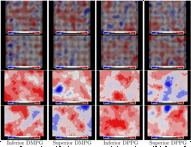
\includegraphics[resolution=100,scale=0.5]{Plots/glomepro/apl_glomepro_1.png}
% \includegraphics[resolution=100,scale=0.1]{Plots/glomepro/snap_15STXrigid-DPPG_1_up.png}
% 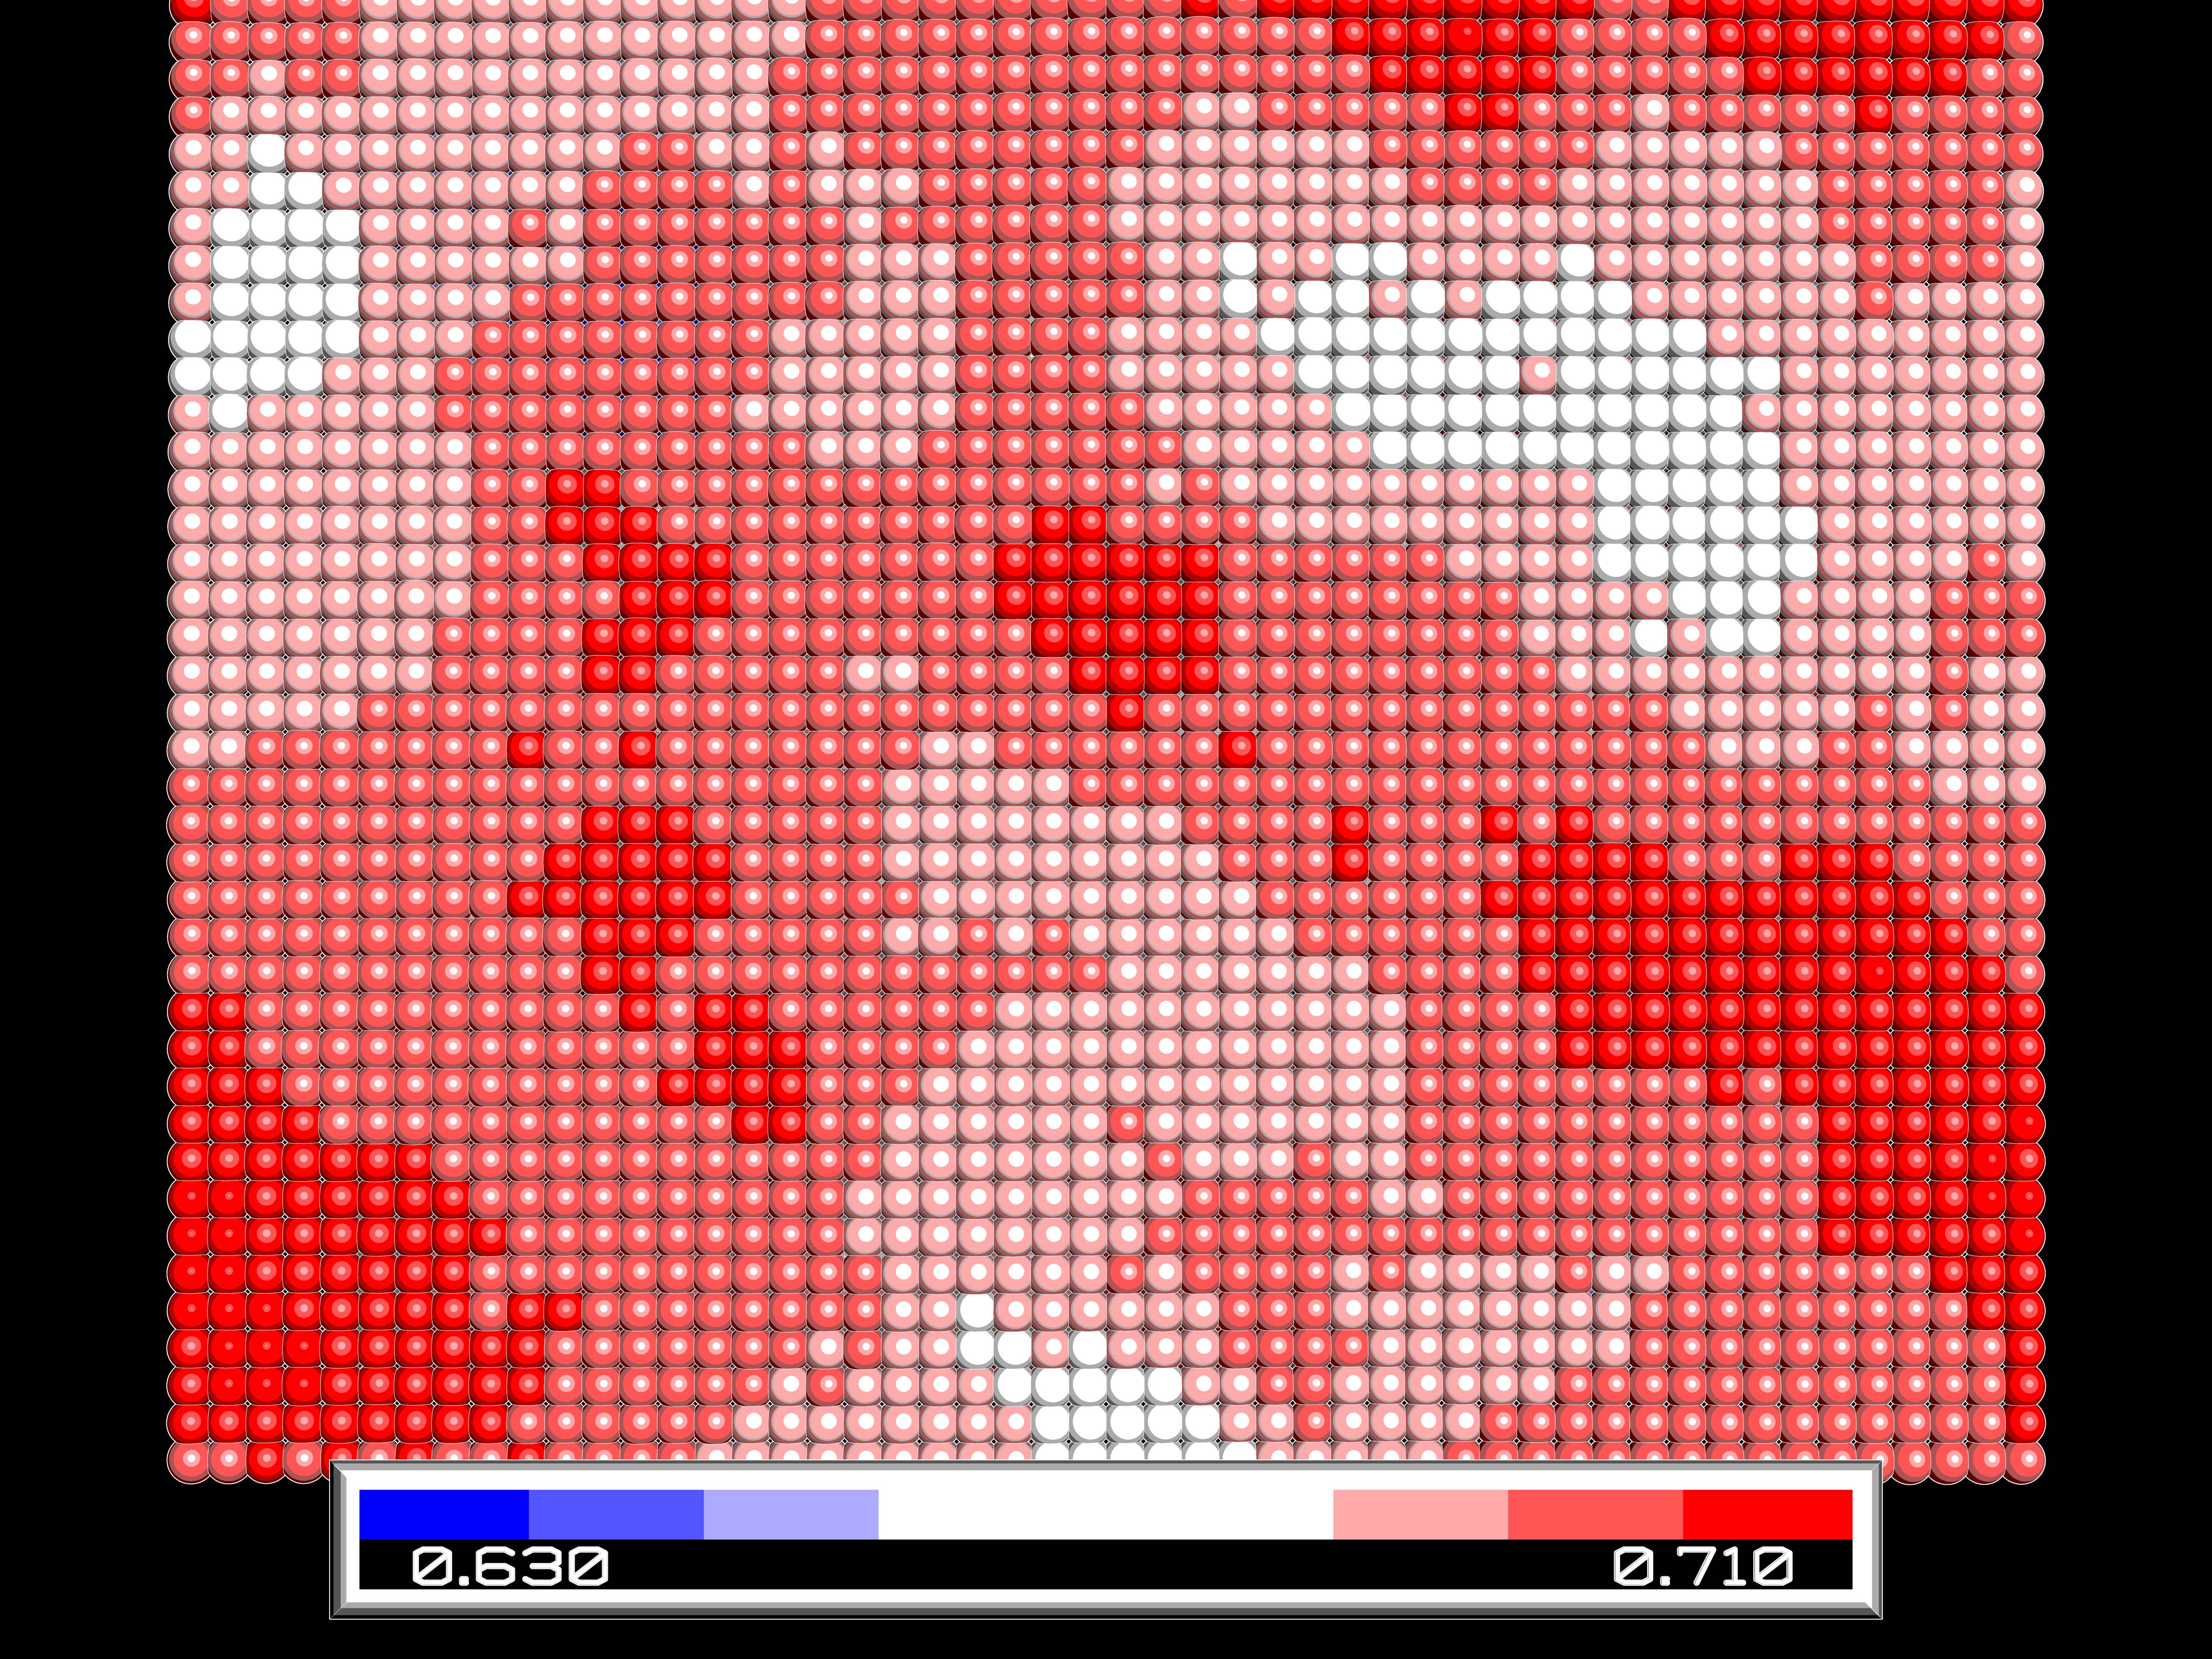
\includegraphics[resolution=100,scale=0.1]{Plots/glomepro/snap_STX-DMPG_1_do.png}
% \includegraphics[resolution=100,scale=0.1]{Plots/glomepro/snap_STX-DMPG_1_up.png}
% \includegraphics[resolution=100,scale=0.1]{Plots/glomepro/snap_STX-DPPG_1_do.png}
% \includegraphics[resolution=100,scale=0.1]{Plots/glomepro/snap_STX-DPPG_1_up.png}
% \includegraphics[resolution=100,scale=0.1]{Plots/glomepro/snap_STXrigid-DMPG_1_do.png}
% \includegraphics[resolution=100,scale=0.1]{Plots/glomepro/snap_STXrigid-DMPG_1_up.png}
% \includegraphics[resolution=100,scale=0.1]{Plots/glomepro/snap_STXrigid-DPPG_1_do.png}
% \includegraphics[resolution=100,scale=0.1]{Plots/glomepro/snap_STXrigid-DPPG_1_up.png}
% \caption{\'{A}rea por l\'{i}pido locales para los sistemas con estafiloxantina. En la figura se muestra la monocapa superior y la inferior.}
\end{center} 
